\section*{BT ÔN TẬP HÀM SỐ - SỐ 3}
\setcounter{ex}{0}\setcounter{bt}{0}
\Opensolutionfile{ans}[ans/ansOC3-CD-1]

\noindent\textbf{I. PHẦN TRẮC NGHIỆM:}
\begin{ex}%[0D2Y1-3]
\immini {Cho hàm số $y=f(x)$ có đồ thị như hình vẽ. Dựa vào đồ thị hàm số $y=f(x)$, mệnh đề nào sau đây \textbf{sai}?
\choice
{Hàm số $y=f(x)$ đồng biến trên khoảng $\left(-\infty;0\right)$}
{\True Hàm số $y=f(x)$ đồng biến trên khoảng $\left(0;+\infty\right)$}
{Hàm số $y=f(x)$ đồng biến trên khoảng $\left(2;+\infty\right)$}
{Hàm số $y=f(x)$ nghịch biến trên khoảng $\left(0;2\right)$}}{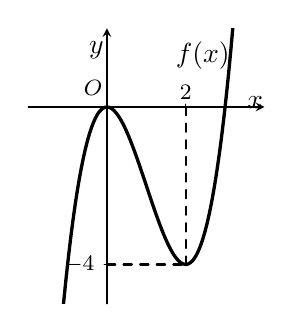
\begin{tikzpicture}[line cap=round,line join=round,>=stealth,x=1.0cm,y=1.0cm, scale=0.5]
\draw[->] (-2.,0.) -- (4.,0.);
\foreach \x in {2}
\draw[shift={(\x,0)}] (0pt,2pt) -- (0pt,-2pt) node[above] {\footnotesize $\x$};
\draw[->] (0.,-5.) -- (0.,2.);
\foreach \y in {-4}
\draw[shift={(0,\y)}] (2pt,0pt) -- (-2pt,0pt) node[left] {\footnotesize $\y$};
\draw (-10pt,1pt) node[above] {\footnotesize $O$};
\clip(-2.,-5.) rectangle (4.,2.);
\draw[line width=1.2pt,smooth,samples=100,domain=-2.0:4.0] plot(\x,{(\x)^(3.0)-3.0*(\x)^(2.0)});
\draw [line width=0.8pt,dash pattern=on 3pt off 3pt] (2.,0.)-- (2.,-4.);
\draw [line width=0.8pt,dash pattern=on 3pt off 3pt] (0.,-4.)-- (2.,-4.);
\draw (3.31,0.5) node[anchor=north west] {$x$};
\draw (1.5,1.9) node[anchor=north west] {$f(x)$};
\draw (-0.7,1.9) node[anchor=north west] {$y$};
\end{tikzpicture}
}
\loigiai{
Dựa vào đồ thị ta có mệnh đề \lq\lq Hàm số $y=f(x)$ đồng biến trên khoảng $\left(0;+\infty\right)$\rq\rq\, là mệnh đề sai.
}
\end{ex}

\begin{ex}%[0D3Y1-2]
    Tìm tập xác định $\mathscr{D}$ của hàm số $y=\dfrac{3x-1}{2x-2}$?
    \choice
    {$\mathscr{D}=\mathbb{R}$}
    {$\mathscr{D}=\left( 1;+\infty \right)$}
    {\True $\mathscr{D}=\mathbb{R} \setminus \left\{ 1 \right\}$}
    {$\mathscr{D}=\left[ 1;+\infty \right)$}
    \loigiai{
        Hàm số xác định khi $2x-2\ne 0\Leftrightarrow x\ne 1$.\\
        Vậy tập xác định của hàm số là $\mathscr{D}=\mathbb{R} \setminus \left\{ 1 \right\}$.
    }
\end{ex}

\begin{ex}%[0D3Y1-2]
    Tìm tập xác định của hàm số $y=\sqrt{x-2}-\sqrt{3+x}$?
    \choice
    {$\mathscr{D}=\left[ -3;+\infty \right)$}
    {\True $\mathscr{D}=\left[ 2;+\infty \right)$}
    {$\mathscr{D}=\mathbb{R}$}
    {$\mathscr{D}=[-3;2]$}
    \loigiai{
        Hàm số xác định khi $\heva{
            & x-2\ge 0 \\ 
            & x+3\ge 0} \Leftrightarrow \heva{
            & x\ge 2 \\ 
            & x\ge -3} \Leftrightarrow x\ge 2$.\\
        Vậy $\mathscr{D}=\left[ 2;+\infty \right)$.
    }
\end{ex}

\begin{ex}%[0D2Y1-3]
\immini{Cho hàm số $y=f(x)$ có đồ thị như hình bên. Kết luận nào sau đây là \textbf{sai}?
\choice
{Hàm số đồng biến trên khoảng $ (0;1)$}
{Hàm số nghịch biến trên khoảng $(1;3) $}
{Hàm số đồng biến trên khoảng $ (3;4) $}
{\True Hàm số đồng biến trên khoảng $(1;4)$}
}{
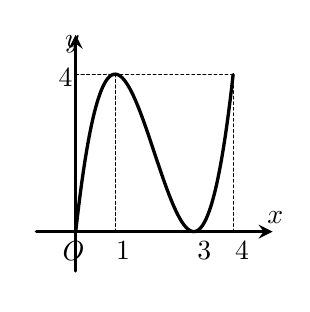
\begin{tikzpicture}[line cap=round,line join=round,>=stealth,scale=.5]
\clip(-1.22,-1.32) rectangle (5.24,5.18);
\draw[line width=1.2pt,domain=0:4,samples=100] plot(\x,{\x^3-6*\x^2+9*\x});
\draw [dash pattern=on 1pt off 1pt] (0.,4.)-- (1.,4.);
\draw [dash pattern=on 1pt off 1pt] (1.,4.)-- (1.,0.);
\draw [dash pattern=on 1pt off 1pt] (4.,4.)-- (4.,0.);
\draw [line width=1.2pt,->] (-1.,0.) -- (5.,0.);
\draw [line width=1.2pt,->] (0.,-1.) -- (0.,5.);
\draw [dash pattern=on 1pt off 1pt] (0.,4.)-- (4.,4.);
\draw [dash pattern=on 1pt off 1pt] (1.,4.)-- (1.,0.);
\draw (4.62,0.76) node[anchor=north west] {$x$};
\draw (-0.52,5.22) node[anchor=north west] {$y$};
\draw (-0.58,0) node[anchor=north west] {$O$};
\draw (0.78,0) node[anchor=north west] {$1$};
\draw (3.8,0) node[anchor=north west] {$4$};
\draw (2.84,0) node[anchor=north west] {$3$};
\draw (-0.68,4.38) node[anchor=north west] {$4$};
\end{tikzpicture}
}
\loigiai{
Vì hàm số nghịch biến trên $(1;3)$ và $(1;3)\subset (1;4)$ nên hàm số không thể đồng biến trên $(1;4)$.
}
\end{ex}

\begin{ex}%[0D3Y1-2]
    Tập xác định của hàm số $y=\dfrac{x-1}{x^2-x+3}$ là
    \choice
    {$\mathscr{D}=\varnothing $}
    {$\mathscr{D}=\mathbb{R}$}
    {$\mathscr{D}=\mathbb{R} \setminus \left\{ 1 \right\}$}
    {$\mathscr{D}=\mathbb{R} \setminus \left\{ 0;1 \right\}$}
    \loigiai{
        Ta có: $x^2-x+3 \ne 0 \Leftrightarrow \forall x\in \mathbb{R}$.\\
    Vậy $\mathscr{D}=\mathbb{R}$.   
    }
\end{ex}


\begin{ex}%[0D2B1-1]
Cho hàm số $f(x)=a(x-m)(x-n)$ có đồ thị đi qua các điểm $A(0; -16), B(4; 0)$ và $C(12; 0)$. Giá trị của $m\cdot n$ là
\choice
{$8$}
{$12$}
{$16$}
{\True $48$}
\loigiai{
Vì đồ thị hàm số đi qua các điểm $(0; -16), (4; 0), (12; 0)$ nên có hệ $\heva{&-16=a (-m) (-n)\\&0=a(4-m)(4-n)\\&0=a(12-m)(12-n).}$\\
Vì $a\neq 0$ nên $\hoac{&m=4\\&n=4}$ và $\hoac{&m=12\\&n=12}$. Suy ra $\heva{m=4\\n=12}$ hoặc $\hoac{&m=12\\&n=4}$. Do đó $m\cdot n=48$.}
\end{ex}

\begin{ex}%[0D2B1-3]
\immini{
Cho hàm số $y=f(x)$ có đồ thị trên đoạn $[-2;4]$ như hình vẽ. Xét trên đoạn $[-2;4]$, mệnh đề nào sau đây là đúng?
\choice
{Hàm số đồng biến trên các khoảng $(-2,2)$ và $(3,4)$}
{Hàm số đạt giá trị nhỏ nhất là $-2$}
{\True Hàm số đạt giá trị lớn nhất là $3$}
{Chỉ có hai giá trị của $x$ thoả mãn $f(x)=1$}}
{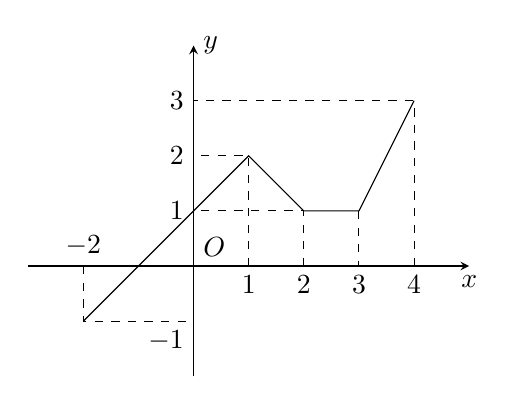
\begin{tikzpicture}[>=stealth,scale=0.7]
\draw[->](-3,0)--(5,0)node[below]{$x$};
\draw[->](0,-2)--(0,4)node[right]{$y$};
\draw[](-2,-1)--(1,2)--(2,1)--(3,1)--(4,3);
\draw[dashed](-2,0)node[above]{$-2$}--(-2,-1)--(0,-1)node[below left]{$-1$};
\draw[dashed](1,0)node[below]{1}--(1,2)--(0,2)node[left]{2};
\draw[dashed](2,0)node[below]{2}--(2,1)--(0,1)node[left]{1};
\draw[dashed](3,1)--(3,0)node[below]{3};
\draw[dashed](4,0)node[below]{4}--(4,3)--(0,3)node[left]{3};
\draw (0,0) node[above right]{$O$};
\end{tikzpicture}}
\loigiai{
Trên đoạn $[-2;4]$ của đồ thị, tồn tại điểm $M(4;3)$ có tung độ cao nhất. Do đó giá trị lớn nhất của hàm số trên đoạn $[-2;4]$ là $3$.
}
\end{ex}

\begin{ex}%[0D2B1-3]
\immini{Hàm số $y=f(x)$ có đồ thị như hình vẽ bên. Hàm số $y=f(x)$ đồng biến trên khoảng nào sau đây?
\choice
{\True $(1;3)$}
{$(-1;1)$}
{$(3;5)$}
{$(1;5)$}}{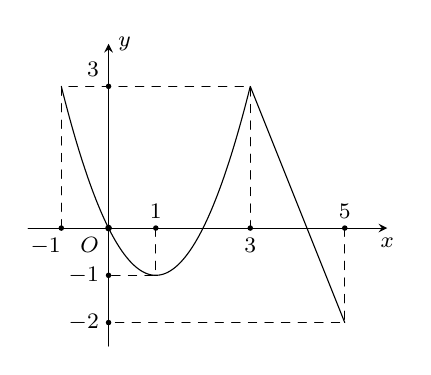
\begin{tikzpicture}[scale=1, font=\footnotesize, line join=round, line cap=round,>=stealth,x=0.6cm,y=0.6cm]
\def \xmin{-1.7};
\def \xmax{5.9};
\def \ymin{-2.5};
\def \ymax{3.9};
\draw[->] (\xmin, 0.) -- (\xmax,0.) node[anchor=north] {$x$};
\draw[->] (0.,\ymin) -- (0.,\ymax) node[anchor=west] {$y$};
\clip(\xmin,\ymin) rectangle (\xmax,\ymax);
\draw[smooth,samples=100,domain=-1:3] plot(\x,{(\x)^2-2*(\x)});
\draw (3,3)--(5,-2);
\draw[dashed] (-1,0) node[below,xshift=-0.2cm] {$-1$} -- (-1,3)--(0,3)node[above left] {$3$} -- (3,3)--(3,0)node[below]{$3$} (1,0) node[above]{$1$}--(1,-1)--(0,-1)node[left]{$-1$} (5,0) node[above]{$5$}--(5,-2)--(0,-2)node[left]{$-2$} ;
\foreach \p/\g in {-1/0,1/0,3/0,5/0,0/-2,0/-1,0/3} \fill[black] (\p,\g) circle(1pt);
\draw[fill=black] (0,0) circle (1pt) node[below left] {$O$};
\end{tikzpicture}}
\loigiai
{Theo đồ thị thì hàm số $y=f(x)$ đồng biến trên khoảng $(1;3)$.
}
\end{ex}

\begin{ex}%[0D2B1-1]
    Cho họ đường thẳng $d_{m}:(m+1)x-2(m-2)y+3=0$ và các mệnh đề
    \begin{enumerate}
        \item $d_{m}$ luôn đi qua hai điểm cố định.
        \item $d_{1}\parallel d_{5}$.
        \item $d_{1}\perp d_{3}$.
        \item $d_{5}$ là đường phân giác thứ nhất của hệ trục tọa độ $Oxy$.
    \end{enumerate}
    Tìm mệnh đề \textbf{sai} trong các mệnh đề trên.
    \choice
    {1}
    {1, 3}
    {2, 3}
    {\True 1,2,3,4}
    \loigiai{
        \begin{enumerate}
            \item Gọi $(x_{0};y_{0})$ là điểm cố định của họ $d_{m}$. Ta có\\
            $m(x_{0}-2y_{0})+(x_{0}+4y_{0}+3)=0$, $\forall m\Leftrightarrow\heva{
                &x_{0}-2y_{0}=0\\
                &x_{0}+4y_{0}+3=0
            }\Leftrightarrow\heva{
                &x_{0}=-1\\
                &y_{0}=-\dfrac{1}{2}
            }$
            \item $d_{1}\colon 2x+2y+3=0$ và $d_{5}\colon 6x-6y+3=0\Rightarrow d_{1}$ không song song với $ d_{5}$.
            \item $d_{1}\colon 2x+2y+3=0$ và $d_{3}\colon 4x-2y+3=0\Rightarrow d_{1}$ cắt $ d_{3}$ và không vuông góc.
            \item $d_{5}\colon 6x-6y+3=0\Rightarrow$ $d_{5}$ không phải là phân giác thứ nhất của hệ tọa độ $Oxy$.
    \end{enumerate} }
\end{ex}

\begin{ex}%[0D2B1-3]
\immini{Cho hàm số $y=f(x)$ có đồ thị như hình vẽ. Hàm số đồng biến trên khoảng nào sau đây?
\choicew{.7\textwidth}
\choice
{$(-2;+\infty)$}
{\True $(0; 3)$}
{$(-2; 0)$}
{$(3; +\infty)$}
}{
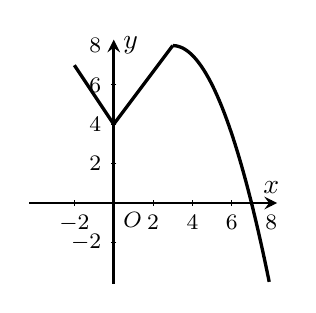
\begin{tikzpicture}[x=0.5cm,y=0.5cm,scale=.5,>=stealth]
\foreach \x in {-2,2,4,6,8}
\draw[shift={(\x,0)},color=black] (0pt,2pt) -- (0pt,-2pt) node[below] {\footnotesize $\x$};
\draw[->,color=black,line width=1pt] (0,-4.1) -- (0,8.3);
\foreach \y in {-2,2,4,6,8}
\draw[shift={(0,\y)},color=black] (2pt,0pt) -- (-2pt,0pt) node[left] {\footnotesize $\y$};
\draw[->,color=black,line width=1pt] (-4.3,0) -- (8.3,0);
\draw[-,smooth,domain=3:7.9,very thick] plot(\x,{-.5*(\x)^2+3*(\x)+3.5});
\draw[smooth,domain=0:3,very thick] plot(\x,{4*(\x/3)+4});
\draw[smooth,domain=-2:0,very thick] plot(\x,{-1.5*(\x)+4});
\draw(0,0)node[below right]{\footnotesize$O$};
\draw(8,0)node[above]{$x$};
\draw(0,8)node[right]{$y$};
\end{tikzpicture}
}
\loigiai{
Dựa vào đồ thị ta thấy hàm số đồng biến trên khoảng $ (0;3) $.
}
\end{ex}

\begin{ex}%[0D2B1-3]
\immini{
Cho hàm số $y=f(x)$ có tập xác định là $[-3;3]$ và đồ thị của nó được biểu diễn bởi hình bên. Khẳng định nào dưới đây là đúng?
\choice
{Hàm số nghịch biến trên khoảng $(1;0)$}
{Hàm số nghịch biến trên khoảng $(0;3)$}
{\True Hàm số nghịch biến trên khoảng $(-1;1)$}
{Hàm số đồng biến trên khoảng $(-1;4)$}
}{
\begin{tikzpicture}
\draw[>=stealth,->] (-2.5,0) -- (3.5,0) node[above]{\scriptsize $x$};
\draw[>=stealth,->] (0,-1.5) -- (0,2.5) node[left]{\scriptsize $y$};
\draw (0,0) node[below left]{\scriptsize $O$};
\draw [thick] (-2,0)--(-1,1)--(1,-1)--(3,2);
\foreach \i in {-2,-1,1,3}
\draw (\i,0.03) -- (\i,-0.03);
\foreach \i in {-1,1,2}
\draw (0.03,\i) -- (-0.03,\i);
\foreach \i in {-2,-1,1,3}
\draw (\i,0) node[below]{\scriptsize $\i$};
\foreach \i in {-1,1,2}
\draw (0,\i) node[right]{\scriptsize $\i$};
\draw [dashed] (-1,0)|-(-1,1) (1,0)|-(0,-1);
\draw [dashed] (3,0)|-(0,2);
\end{tikzpicture}
}
\loigiai{Dựa vào đồ thị hàm số, ta có hàm số nghịch biến trên khoảng $(-1;1)$.}
\end{ex}

\begin{ex}%[0D2B1-1]
Điểm $A(-1;-2)$ thuộc đồ thị hàm số nào sau đây?
\choice
{\True $y=\dfrac{x-1}{2x+3}$}
{$y=x^4-1$}
{$y=\dfrac{x^3-1}{x^2-2}$}
{$y=x^3+3x^2-4x-6$}
\loigiai{
Xét hàm số $y=\dfrac{x-1}{2x+3}$ có $y(-1)=-2\Rightarrow$ Điểm $A(-1; -2)$ thuộc đồ thị hàm số $y=\dfrac{x-1}{2x+3}$.
}
\end{ex}

\begin{ex}%[0D3B1-3]
    Cho hàm số bậc nhất có đồ thị như hình bên. Trong các khẳng định sau, có bao nhiêu khẳng định đúng?
    \immini
    {I. Hàm số đã cho nghịch biến trên $\mathbb{R}$.\\
        II. Hàm số đã cho có tập giá trị là $[-1;1]$.\\
        III. Đồ thị của hàm số đã cho có hệ số góc bằng 1.}
    {
        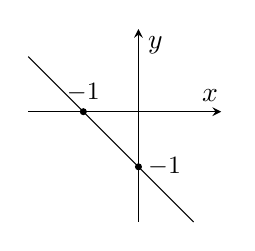
\begin{tikzpicture}[>=stealth,scale=0.7]
            \draw[->] (-2,0) -- (1.5,0);
            \draw (1.3,0.) node [above] {$x$};
            \draw[->] (0,-2)--(0,1.5);
            \draw (0.,1.2) node [right] {$y$};
            \draw (-2,1)--(1,-2);
            \draw[fill] (-1,0)node[above]{\small $-1$} circle (1.5 pt) (0,-1)node[right]{\small $-1$} circle (1.5 pt) ;
        \end{tikzpicture}
    }
    \choice
    {$0$}
    {\True $1$}
    {$2$}
    {$3$}
    \loigiai{
        Đồ thị hàm số là đường thẳng hướng xuống nên hàm số nghịch biến trên $\mathbb{R}$.\\
        Đồ thị hàm số không đối xứng qua gốc tọa độ nên hàm số không là hàm số lẻ.\\
        Đồ thị hàm số hướng xuống nên hệ số góc $a <0$ do đó không bằng 1.
        
    }
\end{ex}

\begin{ex}%[0D2B1-1]
    Biết rằng khi $m$ thay đổi, đồ thị hàm số $y=mx+2m-1$ luôn đi qua một điểm cố định $M_0(a;b)$. Tính tích $T=a\cdot b$.
    \choice
    {$T=1$}
    {\True $T=2$}
    {$T=-2$}
    {$T=-1$}
    \loigiai{
        Điểm cố định là $M_0(-2;-1)$. Vậy $T=2$.
    }
\end{ex}

\begin{ex}%[0D2B1-1]
    Tìm giá trị của $m$ để đồ thị hàm số $y=mx+2$ đi qua điểm $A(1;1)$.
    \choice
    {$m=1$}
    {$m=2$}
    {\True $m=-1$}
    {$m=-2$}
    \loigiai{
        Thay tọa độ $A$ vào phương trình parabol ta được $m+2=1\Leftrightarrow m=-1.$
    }
\end{ex}

\begin{ex}%[0D3B1-3]
    \immini{Đồ thị hình vẽ dưới đây là đồ thị của một hàm số trong bốn hàm số được liệt kê ở bốn phương án $A$, $B$, $C$, $D$ dưới đây. Hỏi hàm số đó là hàm số nào?
        \choice
        {$f(x) = \heva{& 2x - 3 &,x \geq 1\\&x - 2 &,x < 1}$}
        {\True $f(x) = \heva{&2x - 3 &, x < 1\\&x - 2 &,x \geq 1}$}
        {$f(x) = \heva{&3x - 4 &, x \geq 1\\&-x &,x < 1}$}
        {$f(x) = |x - 2|$}}{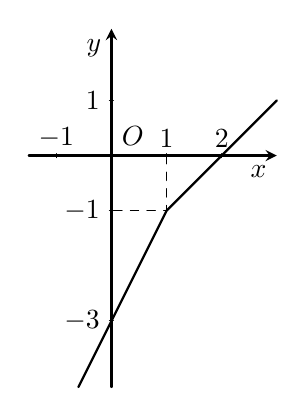
\begin{tikzpicture}[line join=round, line cap=round,>=stealth,thick,scale=.7]
            \tikzset{label style/.style={font=\footnotesize}}
            \def \xmin{-1.5}
            \def \xmax{3}
            \def \ymin{-4.2}
            \def \ymax{2.3}
            \draw[->] (\xmin,0)--(\xmax,0) node[below left] {$x$};
            \draw[->] (0,\ymin)--(0,\ymax) node[below left] {$y$};
            \draw (0,0) node [above right] {$O$};
            \foreach \x in {-1,1,2}
            \draw[thin] (\x,1pt)--(\x,-1pt) node [above] {$\x$};
            \foreach \y in {-3,-1,1}
            \draw[thin] (1pt,\y)--(-1pt,\y) node [left] {$\y$};
            \draw (-0.6,-4.2)--(1,-1)--(3,1);
            \draw[dashed,thin](1,0)--(1,-1)--(0,-1);
        \end{tikzpicture}
    }
    \loigiai{
        \textbf{Trường hợp 1:}  $x < 1$.\\
        Gọi $d \colon y = ax + b$. Khi đó $d$ đi qua điểm $(0; -3)$ và $(1; -1)$ nên ta có hệ $\heva{&b = -3\\&a + b = -1} \Leftrightarrow \heva{&a = 2\\&b = -3.}$\\
        Vậy $d \colon y = 2x - 3$.\\
        \textbf{Trường hợp 2:}  $x \geq 1$.\\
        Gọi $d' \colon y = ax + b$. Khi đó $d'$ đi qua điểm $(2; 0)$ và $(1; -1)$ nên ta có hệ $\heva{&2a + b = 0\\&a + b = -1} \Leftrightarrow \heva{&a = 1\\&b = -2.}$\\
        Vậy $d' \colon y = x - 2$.
    }
\end{ex}

\begin{ex}%[0D3B1-3]
    \immini{Đồ thị hình vẽ là đồ thị của một hàm số trong bốn hàm số được liệt kê ở bốn phương án A, B, C, D dưới đây.
        Hỏi hàm số đó là hàm số nào?
        \choice
        {\True $y=|x|+1$}
        {$y=2|x|+1$}
        {$y=|2x+1|$}
        {$y=|x+1|$}}{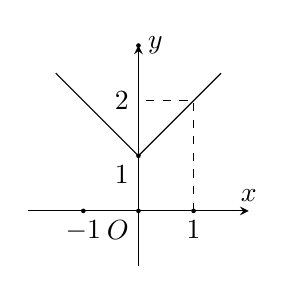
\begin{tikzpicture}[>=stealth,scale=0.7]
            \draw[->](-2,0)--(2,0)node[above]{$x$};
            \draw[->](0,-1)--(0,3)node[right]{$y$};
            \draw[smooth,samples=100,domain=0:1.5]plot(\x,{\x+1});
            \draw[smooth,samples=100,domain=-1.5:0]plot(\x,{-\x+1});
            \draw[dashed](1,0)node[below]{$1$}|-(0,2)node[left]{$2$};
            \fill (-1,0)node[below]{$-1$} circle(1.2pt) (0,0)node[below left]{$O$}circle(1.2pt) (0,1)node[below left]{$1$} circle (1.2pt) (1,0) circle(1.2pt) (0,3)circle(1.2pt);
    \end{tikzpicture}}
    \loigiai{
        Đồ thị hàm số đi qua điểm $(1;2)$.\\
        Đồ thị hàm số không có điểm chung với trục hoành. Nên nhận hàm số $y=|x|+1$.}
\end{ex}

\begin{ex}%[0D3B1-3]
    \immini{
        Đồ thị hình bên là đồ thị của hàm số nào?
        \choice
        {$y=|x|+1$}
        {\True $y=2|x|-1$}
        {$y=|2x-1|$}
        {$y=|x+1|$}
    }{
        \begin{tikzpicture}[>=stealth,font=\footnotesize,scale=0.7]
            \draw[->] (-2,0)--(2.5,0) node[above] {$x$};
            \draw[->] (0,-1.5)--(0,3.5) node[right] {$y$};
            \draw (0,-1)--(1.5,2) (0,-1)--(-1.5,2);
            \draw[dashed] (1,0) node[below] {$1$} |- (0,1) node[left] {$1$};
            \node[below left] at (0,1) {$1$};
            \node[below left] at (0,0) {$O$};
        \end{tikzpicture}
    }
    \loigiai{
        Đồ thị qua điểm $(0;-1)$, suy ra hàm số cần tìm là $y=2|x|-1$.
    }
\end{ex}

\begin{ex}%Câu 1%[0D3B1-2]
    Tìm tập xác định của hàm số $y=\dfrac{\sqrt{x-1}-x}{\sqrt{6-3x}}$?
    \choice
    {$\mathscr{D}=\left[ 1;2 \right)$}
    {\True $\mathscr{D}=\left[ 1;2 \right)$}
    {$\mathscr{D}=\left[ 1;2\right)$}
    {$\mathscr{D}=\left( -\infty ;2 \right)$}
    \loigiai{
        Hàm số xác định khi $\heva{
            & x-1\ge 0 \\ 
            & 6-3x>0 } \Leftrightarrow \heva{
            & x\ge 1 \\ 
            & x<2} \Leftrightarrow 1\le x<2$.\\
        Vậy $\mathscr{D}=\left[ 1;2\right)$.
    }
\end{ex}

\begin{ex}%[0D2B1-1]
    Cho hàm số $y=x^2+bx+c$. Tìm $b, c$ để đồ thị của hàm số đi qua các điểm $A(2;4)$ và $B(-1;-2)$.
    \choice
    {\True $b=1,c=-2$}
    {$b=-1, c=2$}
    {$b=-1,c=-2$}
    {$b=1,c=2$}
    \loigiai{
        Đồ thị hàm số đi qua hai điểm $A(2;4)$ và $B(-1;-2)$ khi và chỉ khi
        $$\heva{&4=4+2b+c \\ &-2=1-b+c} \Leftrightarrow \heva{&b=1 \\ &c=-2.} $$
    }
\end{ex}


\noindent\textbf{II. PHẦN TỰ LUẬN:}
\begin{ex}%[0D3Y1-2]
    Tìm tập xác định của hàm số $y=\dfrac{\sqrt{x+1}}{x-3}$.
    \loigiai{
        Hàm số xác định khi và chỉ khi $\heva{&x+1 \ge 0 \\& x-3 \ne 0} \Leftrightarrow \heva{&x \ge -1\\ &x \ne 3.}$.\\
        Vậy $\mathscr{D}=\left[-1; +\infty \right) \setminus \{3\}$.
    }
\end{ex}

\begin{ex}%[0D3Y1-2]
    Tìm tập xác định của hàm số $y=x+\sqrt{x+4}$.
    \loigiai{
        Hàm số xác định khi và chỉ khi $x+4 \ge 0 \Leftrightarrow x \ge -4$.\\
        Vậy $\mathscr{D}=\left[-4;+\infty\right)$.
    }
\end{ex}

\begin{ex}%[0D3Y1-2]
    Tìm tập xác định của hàm số $y=\sqrt{2-x}$.
    \loigiai{
        Hàm số xác định khi và chỉ khi $2-x \ge 0 \Leftrightarrow x \le 2$.\\
        Vậy $\mathscr{D}=\left( -\infty; 2\right]$.
    }
\end{ex}

\begin{ex}%[0D3Y1-2]
    Tìm tập xác định của hàm số $y=\dfrac{2-x}{x^2-6x+8}$.
    \loigiai{
        Hàm số xác định khi và chỉ khi $x^2-6x+8 \ne 0 \Leftrightarrow \heva{&x \ne 2\\& x \ne 4.}$.\\
        Vậy $\mathscr{D}=\mathbb{R} \setminus \{2;4\}$.
    }
\end{ex}

\begin{ex}%[0D3Y1-2]
    Tìm tập xác định của hàm số $y=-\dfrac{3}{2x-3}$.
    \loigiai{
        Hàm số xác định khi và chỉ khi $2x-3 \ne 0 \Leftrightarrow x \ne \dfrac{3}{2}$.\\
        Vậy $\mathscr{D}=\mathbb{R} \setminus \left\{\dfrac{3}{2}\right\}$.
    }
\end{ex}

\begin{ex}%[0D3B1-2]
    Tìm tập xác định của hàm số $y=-\dfrac{3}{\sqrt{x-2}}+\dfrac{x}{\sqrt{x+2}}$.
    \loigiai{
        Hàm số xác định khi và chỉ khi $\heva{&x-2>0 \\& x+2>0} \Leftrightarrow \heva{&x>2\\ &x>-2} \Leftrightarrow x>2$.\\
        Vậy $\mathscr{D}=\left(2; +\infty \right)$.
    }
\end{ex}

\begin{ex}%[0D3B1-2]
    Tìm tập xác định của hàm số $y=\dfrac{1}{\sqrt{x-1}}+\sqrt{5-x}$.
    \loigiai{
        Hàm số xác định khi và chỉ khi $\heva{&x-1>0 \\& 5-x \ge 0} \Leftrightarrow \heva{&x>1\\ &x \le 5.}$.\\
        Vậy $\mathscr{D}=\left(1; 5\right]$.
    }
\end{ex}

\begin{ex}%[0D3T1-1] 
Một hãng taxi có bảng giá như sau:
\begin{center}
\begin{tabular}{|c|c|c|c|}
    \hline & Giá mở cửa $(0{,}5 \mathrm{~km})$ & Giá cước các kilômét tiếp theo & Giá cước từ kilômét thứ 31 \\
    \hline Taxi 4 chỗ & $11000$ đồng & $14500$ đồng & $11600$ đồng \\
    \hline Taxi 7 chồ & $11000$ đồng & $15500$ đồng & $13600$ đồng \\
    \hline
\end{tabular}
\end{center}
\begin{enumerate}
\item Xem số tiền đi taxi là một hàm số phụ thuộc số kilômét di chuyển, hãy viết công thức của các hàm số dựa trên thông tin từ bảng giá đã cho theo từng yêu cầu:\begin{enumerate}
\item Hàm số $f(x)$ để tính số tiền hành khách phải trả khi di chuyển $x$ km bằng xe taxi 4 chỗ.
\item Hàm số $g(x)$ để tính số tiền hành khách phải trả khi di chuyển $x$ km bằng xe taxi 7 chỗ.
\end{enumerate}
\item Nếu cần đặt xe taxi cho $30$ hành khách, nên đặt toàn bộ xe 4 chỗ hay xe 7 chỗ thì có lợi hơn?
\end{enumerate}
\loigiai{Gọi $x$ là số kilômét hành khách di chuyển $(x \geq 0)$.
    \begin{enumerate}
        \item 
         Khi đã lên taxi 4 chỗ, hành khách luôn phải trả $11000$ đồng dù đi hay không, do đó số tiền phải trả luôn bao gồm $11000$ đồng này.
        \begin{itemize}
     \item       Nếu $0 \leq x \leq 0{,}5$, số tiền phải trả là $11000$ đồng.
    \item    Nếu $0{,}5<x \leq 30$, số tiền phải trả là
        $$
        11000+14500(x-0,5) \text { hay } 3750+14500 x .
        $$
    \item Nếu $x>30$, số tiền phải trả là
        $$
        11000+14500 \cdot(30-0{,}5)+11600(x-30) \text { hay } 90750+11600 x.
        $$
                \end{itemize}
        Tương tự, đối với taxi 7 chỗ, hàm số $g(x)$ có công thức:
        $$
        g(x)= \begin{cases}11000 & \text { với } 0 \leq x \leq 0{,}5 \\ 3250+15500 x & \text { với } 0{,}5<x \leq 30 \\ 60250+13600 x & \text { với } x>30 .\end{cases}
        $$
\item  Khi có 30 hành khách, nếu đặt toàn bộ xe 4 chỗ thì cần đặt 8 xe. Khi đó, số tiền taxi phải trả là: $f_{1}(x)= \begin{cases}8\cdot11000 & \text { với } 0 \leq x \leq 0{,}5 \\ 8(3750+14500 x) & \text { với } 0{,}5<x \leq 30 \\ 8(90750+11600 x) & \text { với } x>30 .\end{cases}$\\
Nếu đặt toàn bộ xe 7 chỗ thì cần đặt 5 xe. Khi đó, số tiền taxi phải trả là:
$$
g_{1}(x)= \begin{cases}5\cdot11000 & \text { với } 0 \leq x \leq 0{,}5 \\ 5(3250+15500 x) & \text { với } 0{,}5<x \leq 30 \\ 5(60250+13600 x) & \text { với } x>30 .\end{cases}
$$
Ta cần so sánh $f_{1}(x)$ với $g_{1}(x)$.
Xét hiệu số $f_{1}(x)-g_{1}(x)$.\\
Khi $0 \leq x \leq 0,5$, ta có:
$$
f_{1}(x)-g_{1}(x)=8\cdot11000-5\cdot11000=33000>0 \text {. }
$$
Do đó $f_{1}(x)>g_{1}(x)$.\\
Nghĩa là khi 30 người di chuyển quãng đường it hơn hoặc bằng $0,5 \mathrm{~km}$ bằng taxi thì đi xe 4 chỗ sẽ tốn nhiều tiền hơn đi xe 7 chỗ.\\
 Khi $0{,}5<x \leq 30$, ta có:
$$
f_{1}(x)-g_{1}(x)=8(3750+14500 x)-5(3250+15500 x)=13750+38500 x .
$$
Vì $x>0$ nên $f_1(x)-g_1(x)>0$ hay $f_1(x)>g_{1}(x)$.
Nghĩa là khi 30 người di chuyển quãng đường trên $0{,}5 \mathrm{~km}$ đến $30 \mathrm{~km}$ bằng taxi thì đi xe 4 chỗ sẽ tốn nhiều tiền hơn đi xe 7 chỗ.\\
Khi $x>30$, ta có:
$$
f_1(x)-g_1(x)=8(90750+11600 x)-5(60250+13600 x)=424750+24800x.
$$
Vi $x>0$ nên $f_1(x)-g_1(x)>0$ hay $f_1(x)>g_1(x)$.
Nghĩa là khi 30 người di chuyển quãng đường từ $30 \mathrm{~km}$ trở đi bằng taxi thì đi xe 4 chỗ sẽ tốn nhiều tiền hơn đi xe 7 chỗ.\\
Từ ba trường hợp trên, ta đưa ra kết luận: Nếu cần đặt xe taxi cho 30 hành khách thì nên đặt toàn bộ xe 7 chỗ sẽ có lợi hơn (tiết kiệm chi phí hơn đặt toàn bộ xe 4 chỗ).\\
\textbf{Giải thích:} Trong tinh huống tính tiền taxi, khi nói kilômét thứ nhất, ta cần hiểu là quãng đường $x$ lấy giá trị từ $0 \mathrm{~km}$ đến $1 \mathrm{~km}$, nghĩa là $0 \leq x \leq 1$ hay $x \in[0 ; 1]$; khi nói kilômét thứ hai nghĩa là $1<x \leq 2$ hay $x \in(1 ; 2] ; \ldots$ và nói kilômét thứ 31 trở đi nghĩa là $x>30$.
        \end{enumerate}
}
\end{ex}

\begin{ex}%[0D3T1-1] 
Gia đình bạn Sơn sống ở tầng ba, bà ngoại của Sơn sống ở tầng sáu thuộc cùng một chung cư cao tầng. Sơn đi bộ từ nhà mình xuống tầng một để lấy thư và đưa lên nhà bà ngoại. Đưa thư cho bà xong, Sơn quay về nhà mình.\\
Đặt $y=h(t)$ là hàm số biểu thị khoảng cách từ vị trí của Sơn đến mặt đất theo thời gian $t$ từ khi bạn ấy bắt đầu đi cho đến khi về lại nhà mình (chọn gốc thời gian là lúc Sơn bắt đầu đi lấy thư).
$\left(C_{1}\right)$ hay $\left(C_{2}\right)$ là đồ thị của hàm số $y=h(t)$ ? Tại sao?
\begin{center}
    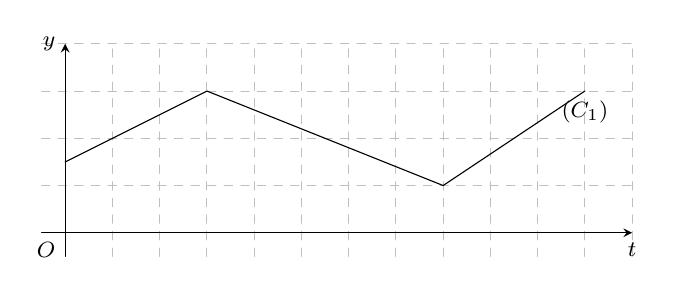
\begin{tikzpicture}[scale=0.6,>=stealth, font=\footnotesize, line join=round, line cap=round]
        \def\a{1} \def\b{-4} \def\c{3} % Hệ số
        \def\xmin{-0.5} \def\xmax{12}
        \def\ymin{-0.5} \def\ymax{4}
        
        \draw[color=gray!50,dashed] (\xmin,\ymin) grid (\xmax,\ymax);
        
        \draw[->] (\xmin,0)--(\xmax,0) node [below]{$t$};
        \draw[->] (0,\ymin)--(0,\ymax) node [left]{$y$};
        \node at (0,0) [below left]{$O$};
        \clip (\xmin+0.1,\ymin+0.1) rectangle (\xmax-0.5,\ymax-0.1);

        \draw(0,1.5)--(3,3)--(8,1)--(11,3)node[below ]{$(C_1)$};
    \end{tikzpicture}
    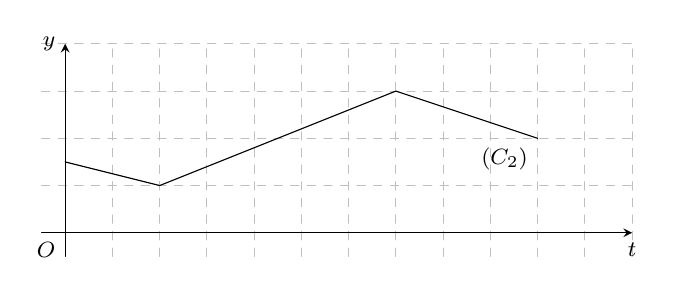
\begin{tikzpicture}[scale=0.6,>=stealth, font=\footnotesize, line join=round, line cap=round]
    \def\a{1} \def\b{-4} \def\c{3} % Hệ số
    \def\xmin{-0.5} \def\xmax{12}
    \def\ymin{-0.5} \def\ymax{4}
    
    \draw[color=gray!50,dashed] (\xmin,\ymin) grid (\xmax,\ymax);
    
    \draw[->] (\xmin,0)--(\xmax,0) node [below]{$t$};
    \draw[->] (0,\ymin)--(0,\ymax) node [left]{$y$};
    \node at (0,0) [below left]{$O$};
    \clip (\xmin+0.1,\ymin+0.1) rectangle (\xmax-0.5,\ymax-0.1);
    
    \draw(0,1.5)--(2,1)--(7,3)--(10,2)node[below left]{$(C_2)$};
\end{tikzpicture}
    \end{center}
\loigiai{
    Khi bắt đầu đi từ tầng ba xuống tầng một, Sơn ngày càng gần mặt đất nên khoảng cách từ vị trí của Sơn đến mặt đất giảm dần, hay hàm số giảm, vậy đồ thị phải có dạng đi xuống.\\
    Khi đi từ tầng một lên tầng sáu để đưa thư cho bà ngoại, Sơn ngày càng xa mặt đất nên khoảng cách từ vị trí của Sơn đến mặt đất tăng dần, hay hàm số tăng, vậy đồ thị phải có dạng đi lên.\\
    Khi đi từ tầng sáu về nhà mình, Sơn ngày càng gần mặt đất nên khoảng cách từ vị trí của Sơn đến mặt đất giảm dần, hay hàm số giảm, vậy đồ thị phải có dạng đi xuống.\\
    Đồ thị $\left(C_{2}\right)$ có dạng tương ứng như mô tả ở trên. Do đó, $\left(C_{2}\right)$ là đồ thị của hàm số $y=h(t)$ này.
}
\end{ex}

\begin{ex}%[0D3T1-1] 
    Bảng giá cước của một hãng Taxi được cho như sau:
    \begin{center}
        \begin{tabular}{|c|c|c|c|c|c|}
            \hline
            \multicolumn{3}{|c|}{\textbf{BẢNG GIÁ CƯỚC}}\\
            \hline
            GIÁ MỞ CỬA & GIÁ KM TIẾP THEO & TỪ KM THỨ $ 31 $\\
            \hline
            $ 11\,000/0{,}7 $ km &$ 15\,800/1 $ km&$ 12\,500/1 $ km\\
            \hline
        \end{tabular}
    \end{center}
    \begin{enumEX}{1}
        \item Gọi $y$ (đồng) là số tiền khách hàng phải trả sau khi đi $x$ (km). Lập hàm số của $y$ theo $x$ (Giả sử không tính thời gian chờ và phí cầu đường bến bãi). 
        \item Một hành khách thuê taxi đi quãng đường $ 40 $ km phải trả số tiền là bao nhiêu? 
    \end{enumEX}
    \loigiai{
        \begin{enumEX}{1}
            \item Nếu quãng đường khách hàng đi không quá $ 0{,}7 $ km, ta có hàm số là: $ y = 11\,000 $.\\
            Nếu quãng đường khách hàng đi trên $ 0{,}7 $ km đến $ 30 $ km, ta có hàm số là:\\
            $ y = 11\,000 + (x - 0{,}7) \cdot 15\,800 = 15\,800 \cdot x - 60 $.\\
            Nếu quãng đường khách hàng đi trên 30km, ta có hàm số là:\\ 
            $ y = 11\,000 + (30 - 0{,}7) \cdot 15\,800 + (x - 30) \cdot 12\,500 = 12\,500 \cdot x + 98\,940 $. 
            \item Thay $ x = 40 $ vào công thức $ y = 12\,500 \cdot x + 98\,940 $ (vì $ 40\text{\;km} > 30\text{\;km} $), ta được:\\
            $ y = 12\,500 \cdot 40 + 98\,940 = 598\,940 $.\\
            Vậy hành khách phải trả số tiền là $ 598\,940 $ đồng.
        \end{enumEX}
    }
\end{ex}

\begin{ex}%[0D3T1-1] 
 Sau khi đun nóng băng phiến lên đến gần $90^{\circ} \mathrm{C}$, người ta để nguội, quan sát, ghi nhận nhiệt độ và trạng thái của băng phiến sau mỗi phút như Bảng 1.\\
Bảng 1. Nhiệt độ và trạng thái của băng phiến khi để nguội
\begin{center}
\begin{tabular}{|l|l|l|l|l|l|l|l|l|l|l|l|}
    \hline Thời gian nguội (phút)& 0 & 1 & 2 & 3 & 4 & 5 & 6 & 7 & 8 & 9 & 10 \\
    \hline Nhiệt độ $\left({ }^{\circ} C\right)$ & 86 & 84 & 82 & 81 & 80 & 80 & 80 & 80 & 79 & 77 & 75 \\
    \hline Trạng thái & \multicolumn{3}{c|}{ lỏng } & \multicolumn{3}{c|}{ lỏng và rắn } & \multicolumn{5}{c|}{ rắn } \\
    \hline
\end{tabular}
\end{center}
\begin{enumerate}
\item Tại sao từ bảng trên, có thế nói nhiệt độ của băng phiến là một hàm số theo thời gian (nung nóng)? Tìm tập xác định và tập giá trị của hàm số trên.
\item Sau khi để nguội 3 phút, nhiệt độ băng phiến là bao nhiêu?
\item Băng phiến chuyển hoàn toàn sang trạng thái rắn sau bao nhiêu phút?
\end{enumerate}
\loigiai{
    \begin{enumerate}
    \item Bảng giá trị cho thấy nhiệt độ (kí hiệu là $y$) là một hàm số theo thời gian (kí hiệu là $x$) vì khi cho $x$ một giá trị bất kì, ta luôn tìm được duy nhất một giá trị của $y$. Do vậy bảng này xác định một hàm số biểu thị nhiệt độ của băng phiến theo thời gian.
    \item Từ bảng giá trị của hàm số, ta có tập xác định $D=\{0 ; 1 ; 2 ; 3 ; 4 ; 5 ; 6 ; 7 ; 8 ; 9 ; 10\}$ và tập giá trị $T=\{75 ; 77 ; 79 ; 80 ; 81 ; 82 ; 84 ; 86\}$.
    \item Sau khi để nguội 3 phút, nhiệt độ băng phiến là $81{ }^{\circ} \mathrm{C}$.
    \item Băng phiến chuyển hoàn toàn sang trạng thái rắn sau 8 phút (lúc đó nhiệt độ băng phiến là $79^{\circ} \mathrm{C}$).
\end{enumerate}
}
\end{ex}

\begin{ex}%[0D3T1-1] 
Trong kinh tế thị trường, lượng cầu và lượng cung là hai khái niệm quan trọng. Lượng cầu chỉ khả năng về số lượng sản phẩm cần mua của bên mua (người tiêu dùng), tuỳ theo đơn giá bán sản phẩm; còn lượng cung chỉ khả năng cung cấp số lượng sản phẩm này cho thị trường của bên bán (nhà sản xuất) cũng phụ thuộc vào đơn giá bán sản phẩm.\\
Người ta khảo sát nhu cầu của thị trường đối với sản phẩm $\mathrm{A}$ theo đơn giá của sản phẩm này và thu được bảng sau:
\begin{center}
\begin{tabular}{|c|c|c|c|c|c|}
    \hline Đơn giá sản phẩm A (đơn vị: nghìn đồng) & 10 & 20 & 40 & 70 & 90 \\
    \hline Lượng cầu (nhu cầu về số sản phẩm) & 338 & 288 & 200 & 98 & 50 \\
    \hline
\end{tabular}
\end{center}
\begin{enumerate}
\item Hãy cho biết tại sao bảng giá trị trên xác định một hàm số? Hãy tìm tập xác định và tập giá trị của hàm số đó (gọi là hàm cầu).
\item Giả sử lượng cung của sản phẩm $\mathrm{A}$ tuân theo công thức $y=f(x)=\dfrac{x^{2}}{50}$, trong đó $x$ là đơn giá sản phẩm $\mathrm{A}$ và $y$ là lượng cung ứng với đơn giá này. Hãy điền các giá trị của hàm số $f(x)$ (gọi là hàm cung) vào bảng sau:
\begin{center}
\begin{tabular}{|c|l|l|l|l|l|}
    \hline Đơn giá sản phầm $\mathrm{A}$ (đơn vị: nghìn đồng) & 10 & 20 & 40 & 70 & 90 \\
    \hline Lượng cung (khả năng cung cấp về số sản phẩm) & & & & & \\
    \hline
\end{tabular}
\end{center}
\item Ta nói thị trường của một sản phẩm là \textit{cân bằng} khi lượng \textit{cung }và lượng \textit{cầu} bằng nhau. Hãy tìm đơn giá $x$ của sản phẩm  A khi thị trường cân bằng.
\end{enumerate}
\loigiai{\begin{enumerate}
    \item Có thể thấy với mỗi mức đơn giá, đều có duy nhất một giá trị về lượng cầu. Do vậy bảng giá trị cho ở đề bài xác định một hàm số.
    Hàm số có tập xác định $D=\{10 ; 20 ; 40 ; 70 ; 90\}$ và tập giá trị
    $$
    T=\{338 ; 288 ; 200 ; 98 ; 50\} .
    $$
    \item
    \begin{tabular}{|c|c|c|c|c|c|}
        \hline Đơn giá sản phẩm A (đơn vị nghìn đồng) & 10 & 20 & 40 & 70 & 90 \\
        \hline Lượng cung (khả năng cung cấp về số sản phẩm) & 2 & 8 & 32 & 98 & 162 \\
        \hline
    \end{tabular}
    \item Dựa vào hai bảng giá trị của lượng cung và lượng cầu, ta tìm được giá trị $x=70$ thì lượng cung và lượng cầu đều bằng $98$. Vậy thị trường của sản phẩm A cân bằng khi đơn giá của sản phẩm A này là $70000$ (đồng).
\end{enumerate}
}
\end{ex}
\Closesolutionfile{ans}